\chapter{Include using pdfpages}
Include the whole pdf with all pages and some scale down to have our own page numbering.
The pdf has been created from a website using the ``print to pdf'' feature of the \textbf{firefox} web browser which by the way has a very nice pdf viewer with annotation features.
\lstset{language=[LaTeX]TeX}
\begin{lstlisting}[caption={code to include next pages as pdf}]
 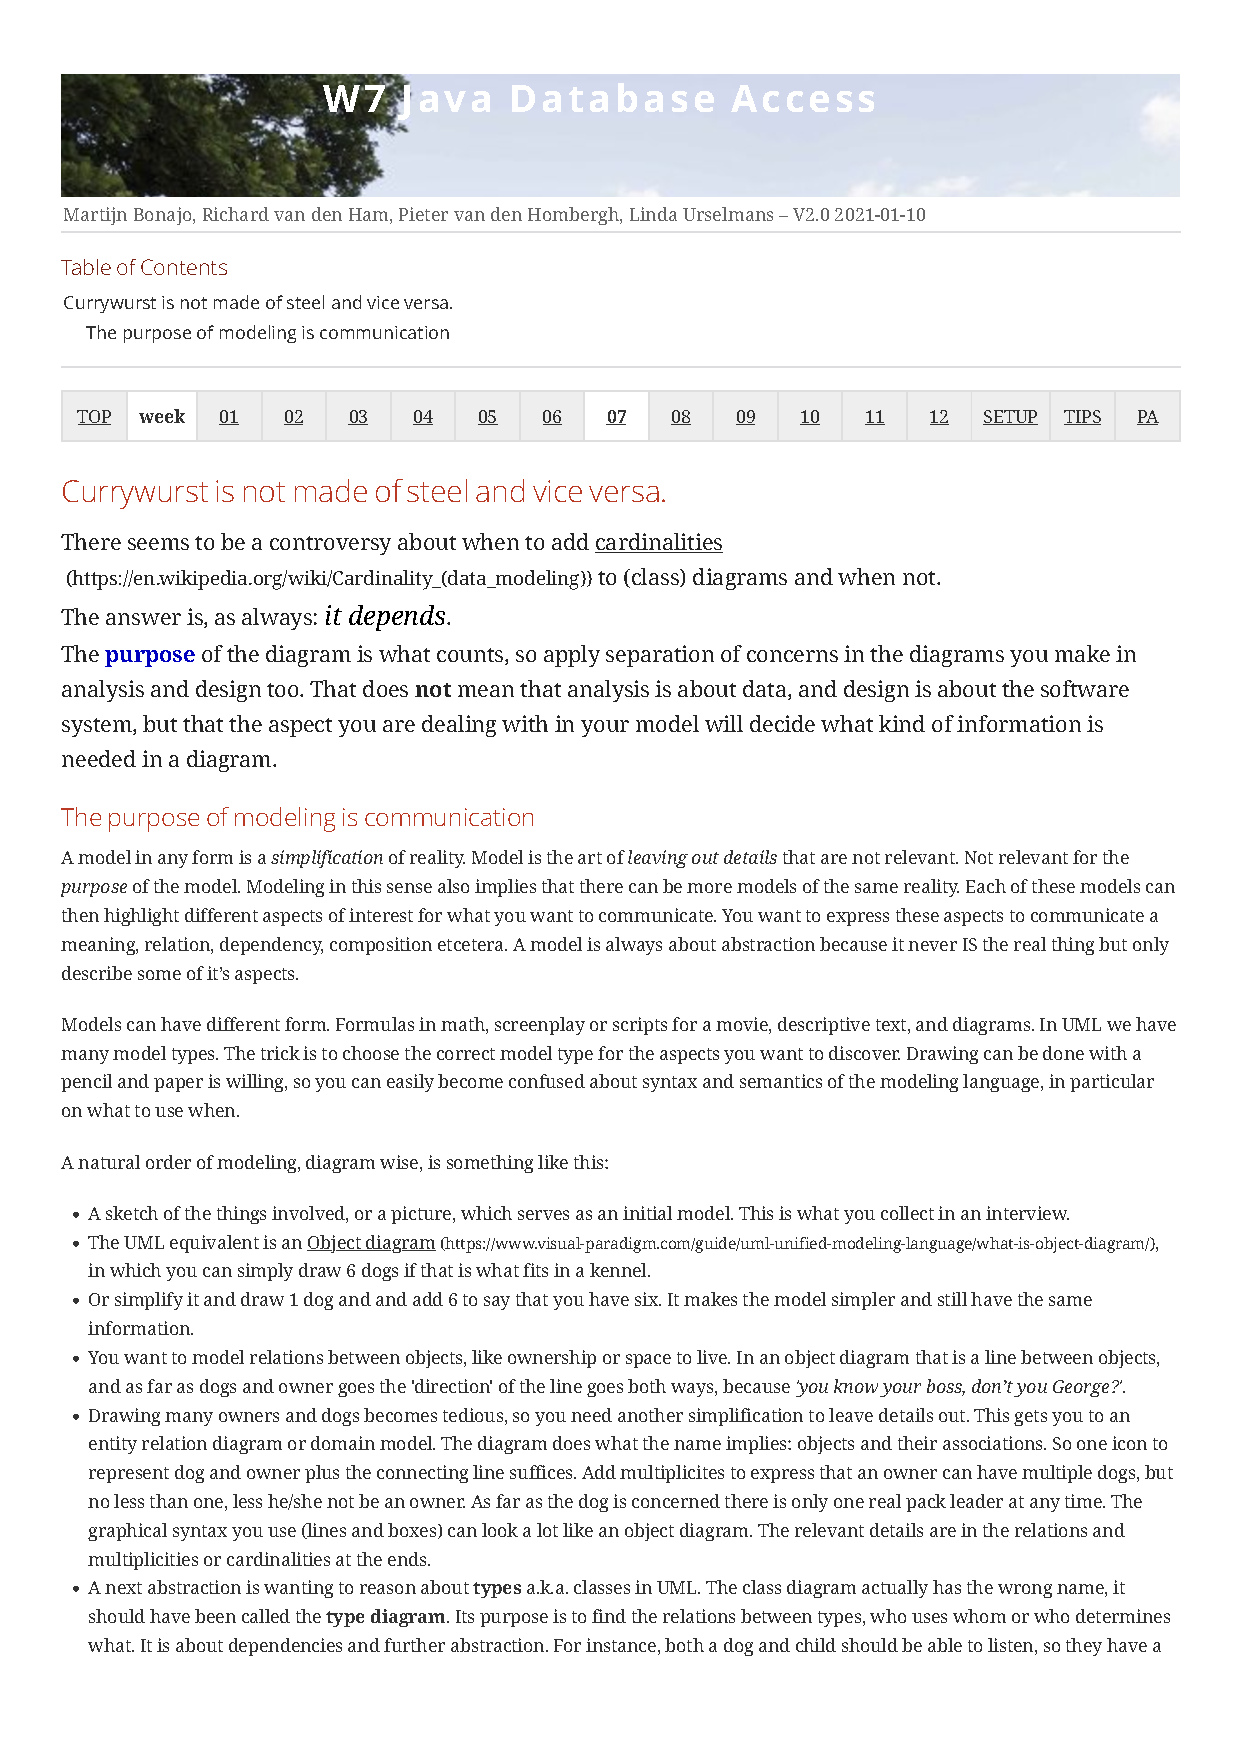
\includepdf[scale=0.9,pages=-,pagecommand={\pagestyle{fancy}}]{appendix/sausageisnotsteel.pdf}
\end{lstlisting}

If you make the documents intended for the appendix in \LaTeX\ too, you should of course simply $\backslash$include them in your report, as all but the last appendix here have been done.

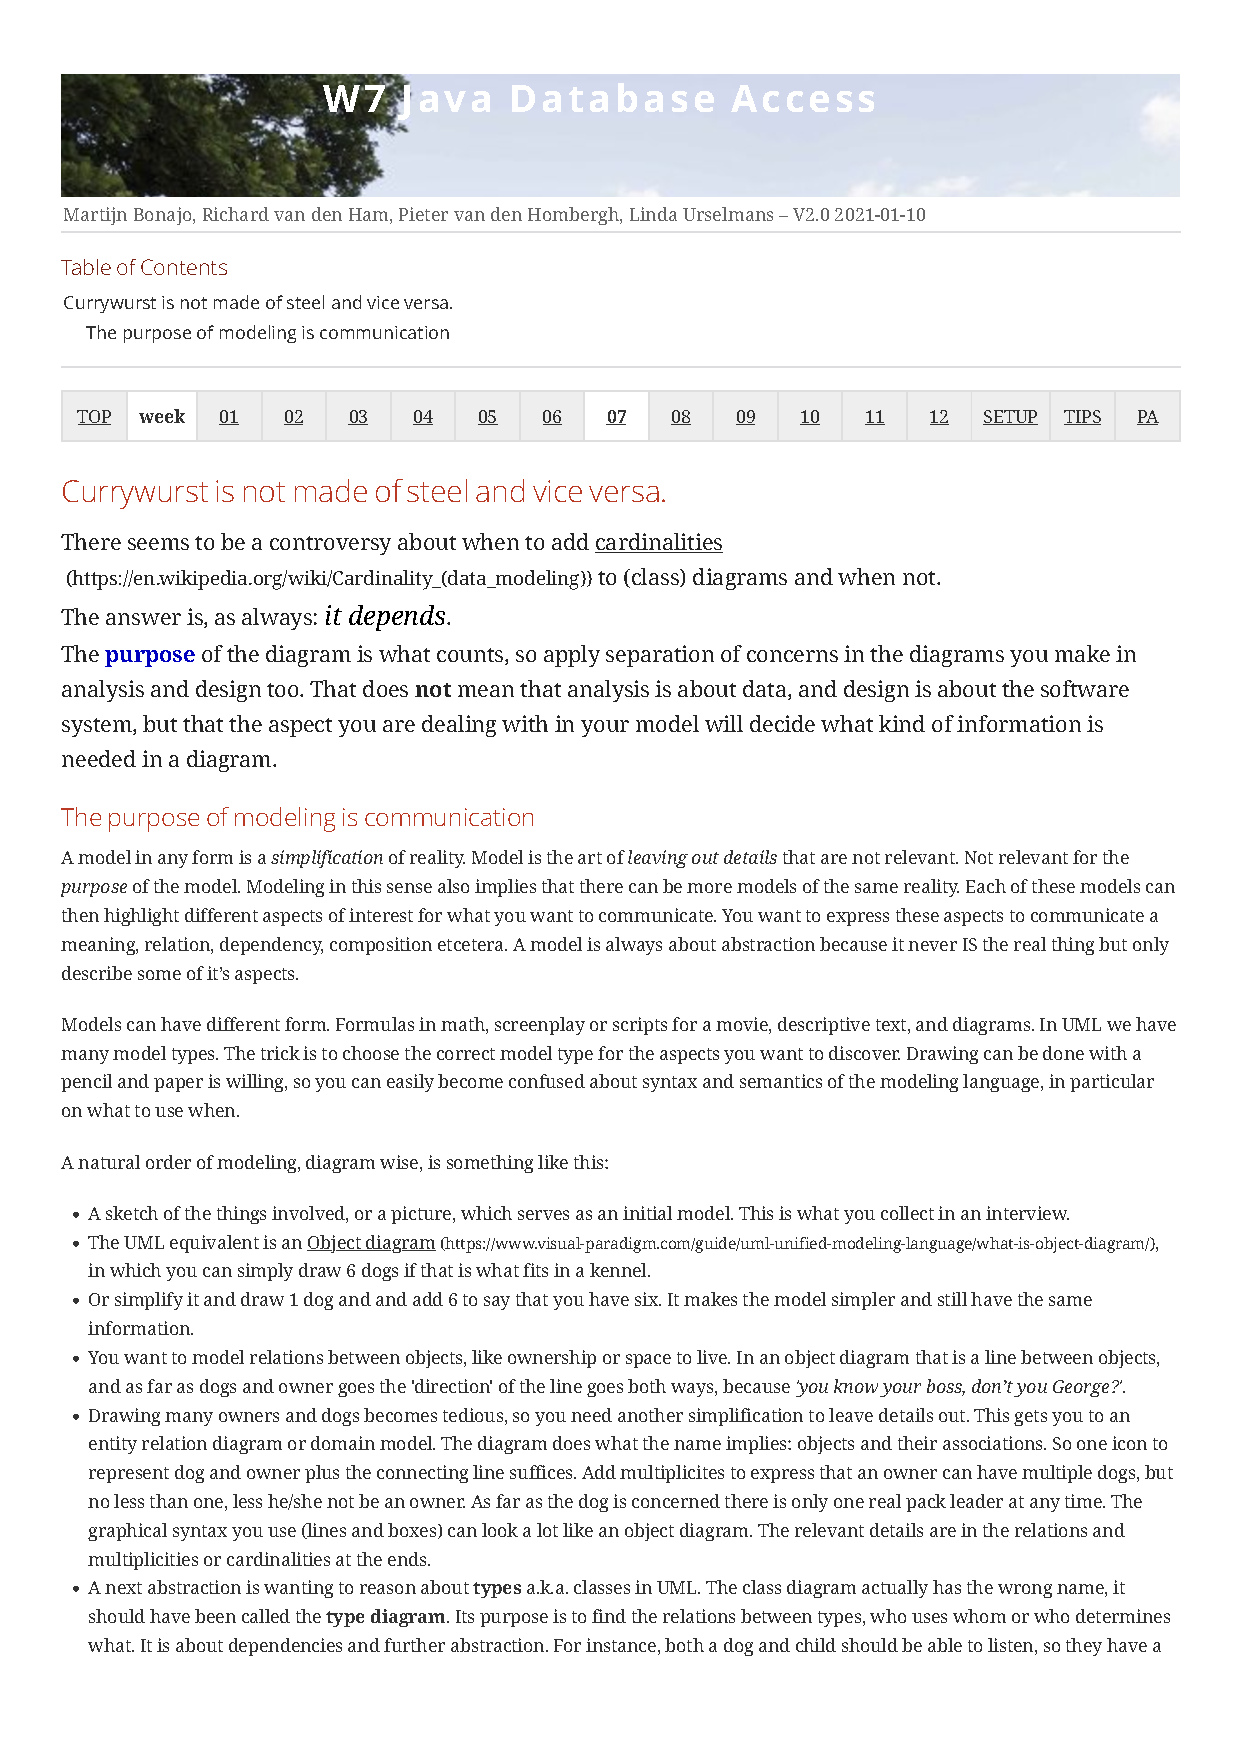
\includepdf[scale=0.9,pages=-,pagecommand={\pagestyle{fancy}}]{appendix/sausageisnotsteel.pdf}

